\vspace{10pt}
\section{Preliminaries}\label{sec:preliminary}

This section provides some preliminaries on ReRAM technology and cross-point architecture. Then the limitations of cross-point architecture are discussed, which motivates the work in this paper.

%demonstrated by a series of simple example, which motivates the work in this paper.

\subsection{Background of ReRAM technology}
Table.~\ref{table:compare} compares the state-of-art non-volatile memory technologies. Obviously, the ReRAM and STT-RAM are the most promising technologies because they have faster access time than PCM and FeRAM with reasonable endurance. However, although the STT-RAM shows the fastest read/write latency among all non-volatile memory technologies, the structure of the memory cell is complex and it has large cell size. On the other hand, the ReRAM has very simple cell structure and can be implemented as a cross-point structure, which can work without access devices. The easy structure provides the possibility of high density integration and 3-D stackability to ReRAM based memory. Besides, the ReRAM also has much higher ON-OFF resistance ratio than STT-RAM. Therefore, with all of these advantages, ReRAM based memory is a highly competitive
technology compared to all of the emerging non-volatile memory technologies.

\begin{table}[!b]
  \centering
  \scriptsize
    \scriptsize
  \caption{Comparison of Non-Volatile Memory Technologies}\label{table:compare}
  \vspace{-5pt}
%  \begin{tabular}{|cccccp{3.5cm}|}
  \begin{tabular}{|c|cccc|}
    \hline
    % after \\: \hline or \cline{col1-col2} \cline{col3-col4} ...
    \textbf{Metric} & \textbf{STT-RAM} & \textbf{PCM}    & \textbf{FeRAM} & \textbf{ReRAM}
    \\\hline
    \textbf{Cell Size($F^2$)} & $6-20$ & $4-8$ & $15$ & $4$\\\hline
    \textbf{Read Latency(ns)} &  1-10 & 20-50 & 20-80 & 5-50\\\hline
    \textbf{Write Latency(ns)} & 2-20& 150& 100& 5-50\\\hline
    \textbf{Endurance} &  $10^{15}$ & $10^8$ & $10^{12}$ & $10^{8-10}$\\\hline
  \end{tabular}
  \vspace{-10pt}
\end{table}


%Different from the traditional memory technologies, which use the electron stored in the cell to represent the information, the non-volatile memory use the the phase/state/resistance of the memory cell itself to store the data. Therefore, the nonvolatile memory can retain the stored information without pow supply. This kind of non-volatility make it a potential candidate as the alternative memory technology to replace the DRAM even SRAM technologies.
As implied by the name, the ReRAM uses its resistance to represent the stored information. The resistance of a ReRAM cell can be switched between high resistance state (HRS) and low resistance state (LRS) by applying an external voltage across the cell. The resistance switching behavior has been noticed for several years and attracted great research interest recently for the potential application as next generation non-volatile memory technology. Generally, the ReRAM memory cell is usually built on a Metal-Insulator-Metal (MIM) structure. The resistance switching behaviors have been observed in many MIM nanodevice with different metal oxide materials. For example, a $TiO_2$ based MIM structure ReRAM was proposed by HP Labs in 2008~\cite{memristor:missing}. The proposed ReRAM is considered as the first experimental realization and a theoretical model of the fourth fundamental circuit elements, which is predicted by Chua~\cite{memristor:chua} about 40 years ago. The memristor-based ReRAM has a very small cell size of $50\times50 nm^2$ with access time less than 50ns. Another $HfO_2$-based bipolar ReRAM is implemented by ITRI this year with as small as 7.2ns access time~\cite{memristor:ISSCC2011_ITRI}.

%The memristor based ReRAM built by HP Labs has a two-terminal, two-layer structure. The top and the bottom electrodes are nanowires made by Pt. Two layers of titanium dioxide are sandwiched between these two electrodes in
%a crossbar architecture. By applying an external voltage across the cell, the memristor can switch between two stable states: ON
%state with low resistance and OFF state with high resistance. A
%positive voltage above a specific threshold will switch the device
%into the OFF state (SET operation) and a negative voltage of the
%same magnitude toggles it to its ON state (RESET operation). T

Although there are several different ReRAM proposed by researchers, all of them can be classified into two types: the unipolar ReRAM and the bipolar ReRAM. For a unipolar ReRAM cell, the resistance switching behaviors do not depend on the polarity of the voltage input across the cell and only relate to magnitude and latency of the voltage input. However, for a bipolar ReRAM, the voltage polarity for a ON-to-OFF switching (RESET operation) is different from a OFF-to-ON switching (SET operation). A unipolar ReRAM can be easily stacked on top of a diode to built a one diode one resistor (1D1R) ReRAM. However, as mentioned, the its SET and RESET operations have different latencies and therefore the performance is mainly determined by the longer voltage pulse. Besides, the control of SET, RESET and read operations without any disturbance is another crucial design challenge, especially in the high speed ReRAM design. Therefore, the reported state-of-art high performance ReRAM technologies are dominated by bipolar ReRAM~[\textbf{? Added reference here}].

\subsection{Cross-Point Architecture}
There are two possible memory structures for ReRAM implementation: the traditional MOSFET-accessed structure and the cross-point structure. In the MOS-accessed memory array, the conventional memory cell is substituted by the ReRAM cell where the access device remains to be the MOSFET. In this structure, each ReRAM cell has to be accompanied with a MOSFET access device, whose size is much larger than the ReRAM cell. In this case, the area of the memory array is mainly dominated by MOSFET access device rather than the actual ReRAM cell. Therefore, the ReRAM's advantage of ultra small cell size will be eliminated.

On the contrary, the cross-point structure is more area-efficient for the ReRAM based memory array~\cite{memristor:Cong}. A schematic view of a typical cross-point memory array is shown in Figure.~\ref{fig:array}(a). It can be seen that in the cross-point array, the only item at each crossing point is the ReRAM cell. Therefore, the area of the array is significantly reduced since the large MOSFET access part is removed. Figure.~\ref{fig:array}(b) shows that the cell size of the cross-point memory can achieve $4F^2$, the theoretical minimum size for a single layer single level memory cell. Besides, as aforementioned, the good stackability and the high resistance ratio provide the capability of building multi-layer multi-level cross-point ReRAM array, which can further increase the area efficiency of the ReRAM array~\cite{memristor:ISSCC2011_ITRI}~\cite{memristor:IEDM08_3D}.

For the cross-point structure, the write operation can either write one bit per time or write several bits at the same word line at the same time. Although the second scheme is more efficient, it required a two-step writing methodology to prevent the unintended writing, which will reduce the write speed. Besides, the unselected word line and bit line can be either left floating or half biased. In read operation, two ways are exhibited for preventing a read failure: the first is to supply the same voltage to the unselected row and selected column. In this way, only the data on the select row is read from the selected column. The disadvantage of this method is the voltage drop on the crossing points of the unselected row and the selected column may not be ideal zero because of the resistance of interconnect wires, and this imposes a limitation on the array size. The second way is a two-step read operation. The disturbance current of the partial selected cell on there selected column will be read out beforehand as a background current. Later the total current, comprised of both partial selected cell and full selected cell, will be read out. The state of the selected cell can then be determined by computing the difference between the total current and background current. Since there are different read/write schemes as well as the array size can be chosen for the cross-point array, it is not a easy way to figure out how to design a workable memory array with the minimum area and energy consumption overhead. Thus, following sections will proposed a worst case based methodology to help designer make the choice at the early step of the design.
\begin{figure}
\centering
  % Requires \usepackage{graphicx}
  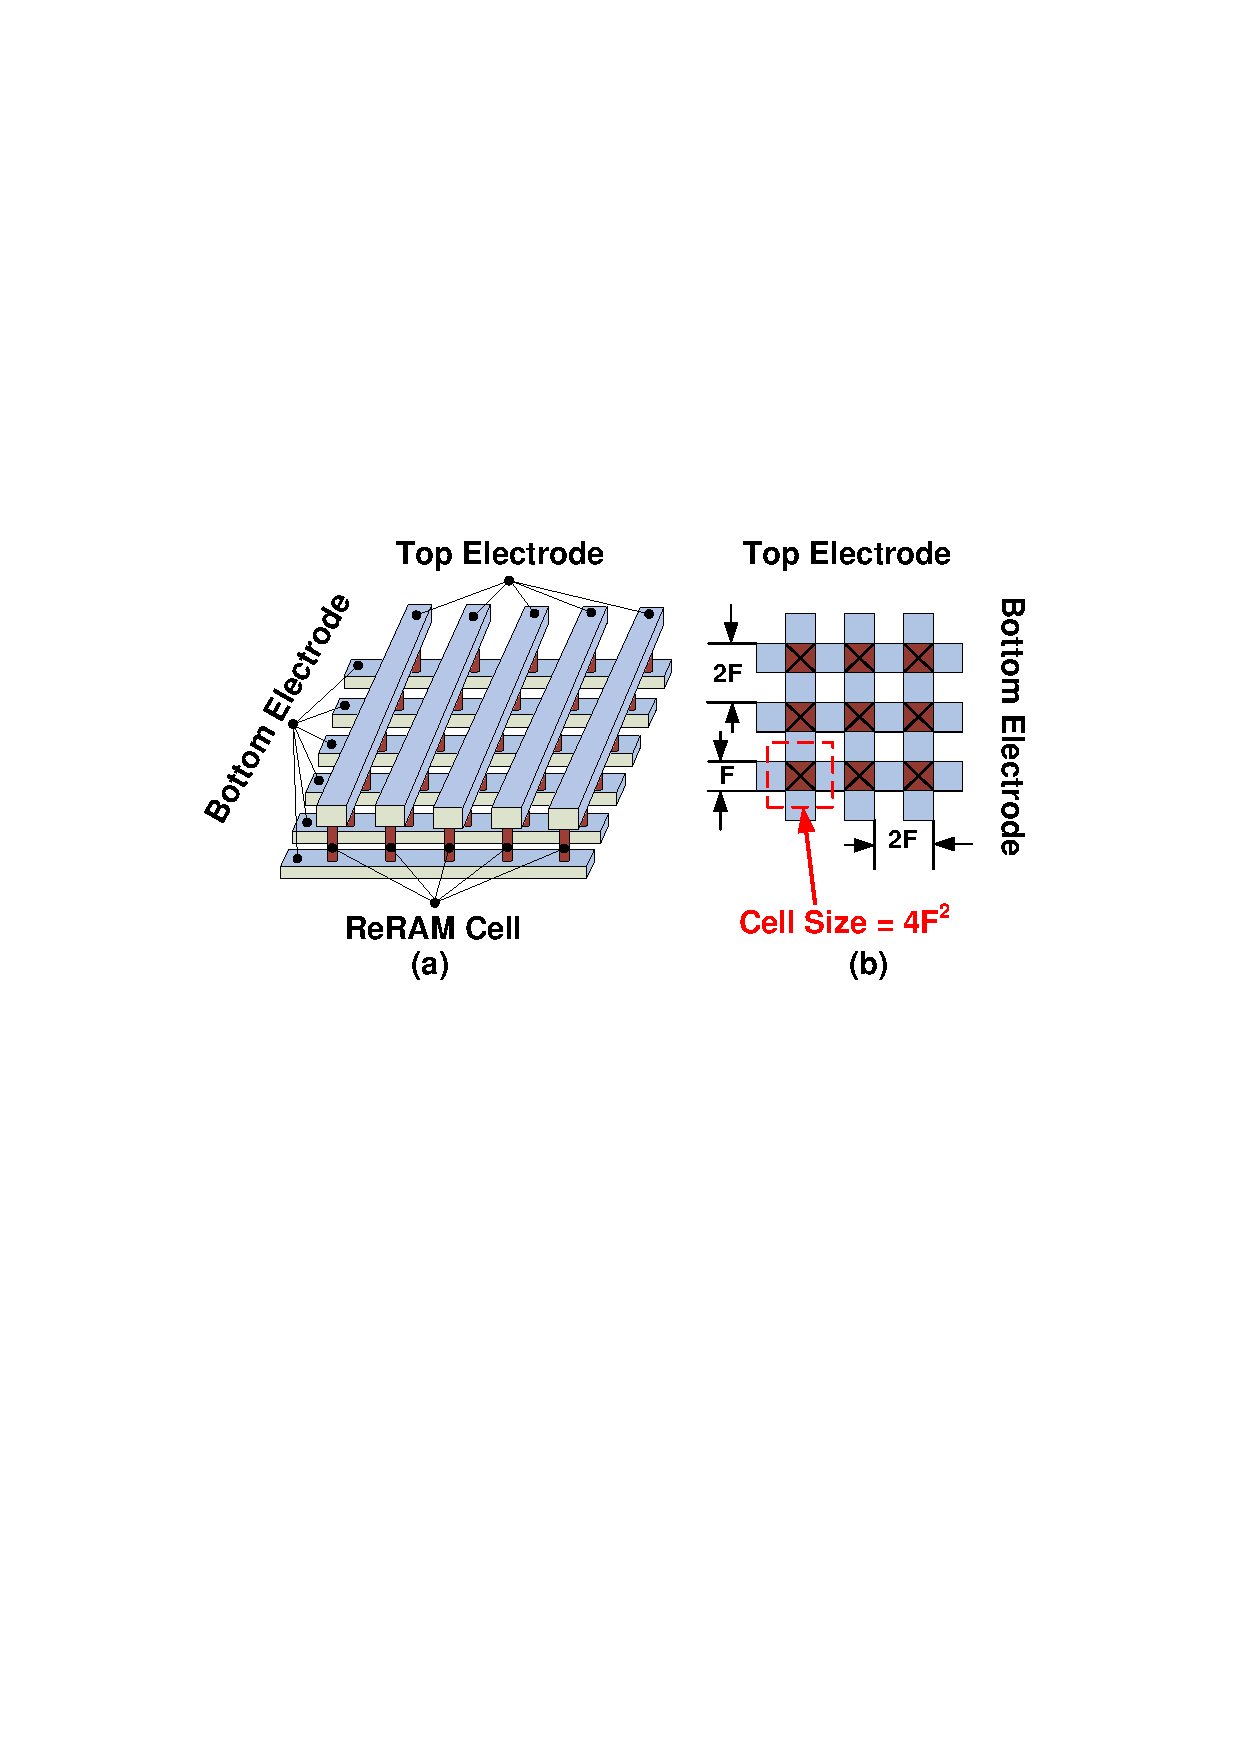
\includegraphics[width=0.45\textwidth]{./figures/crossbar_array2.pdf}\\
  \caption{A schematic view of typical cross-point architecture.}\label{fig:array}
\vspace{-10pt}
\end{figure}

\subsection{Limitations of Cross-Point Architecture}
%\subsection{Related Work and Motivations}
%Although the cross-point structure can provide the fabricate simplicity and area efficiency, it also incur lots of design challenges. Many of the design challenges, such as the array size, resistance ratio as well as the data pattern have been presented and analyzed by previous researches. However, all of these researches focus on the cross point array itself and do not take into account the area or energy overhead of the peripheral circuit. Besides, a comprehensive study on different write/read schemes is also lacking. In this
%
%
%One of the well known design challenge of cross-point is the sneak path existed in the memory array, which will lead a read failure during the read operation and bring in extra energy consumption. Besides, there are also several design options can be chose during the system design. Following shows an example, which shows part of the design challenges of the cross-point structure motivates the work in this paper.
%\begin{enumerate}
%  \item \textbf{Example of the Design Challenges of Cross-Point Structure.}\\
%  In order to
%
%\begin{figure}
%\centering
%  % Requires \usepackage{graphicx}
%  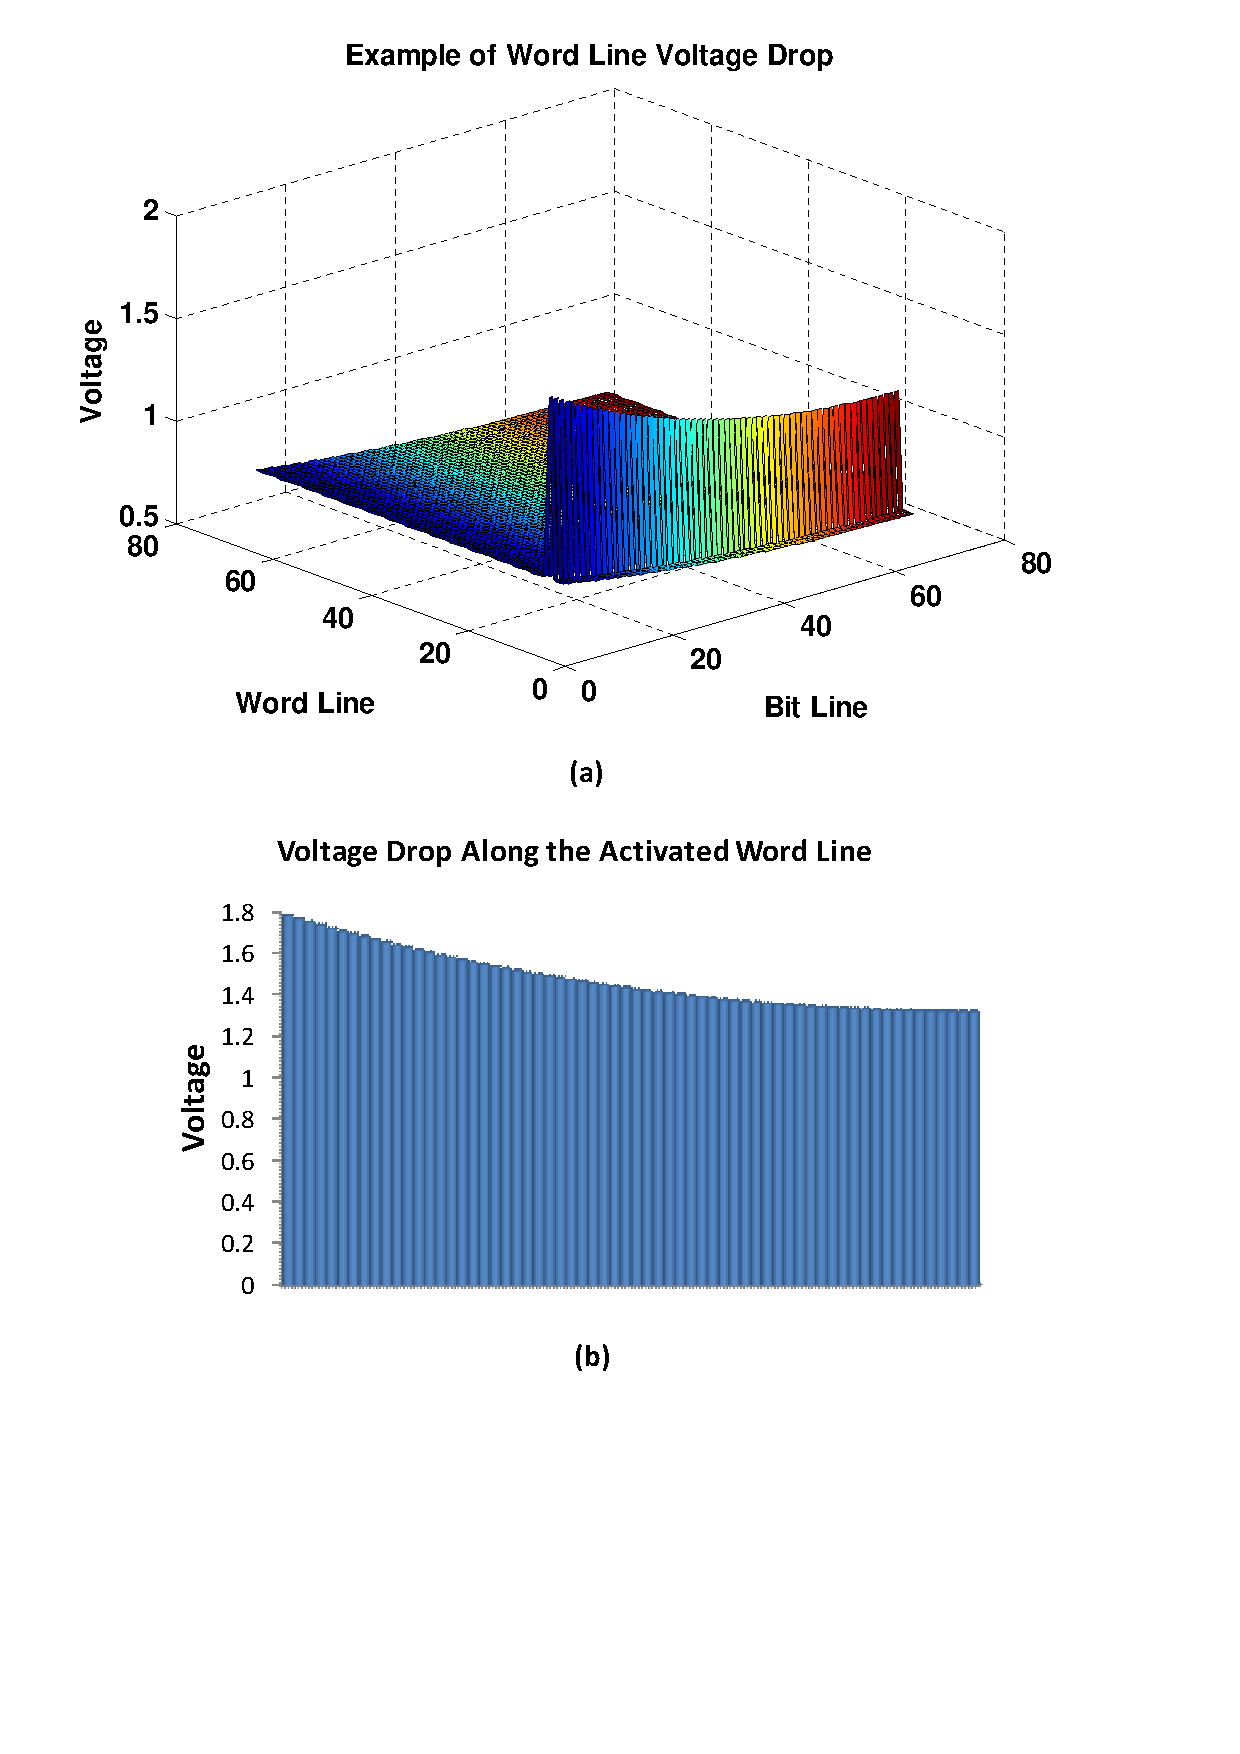
\includegraphics[width=0.4\textwidth]{./figures/example1_large.pdf}\\
%  \caption{Case 1: Voltage Drop Along the Word Line during Write Operation.}\label{fig:exampl1}
%\end{figure}
%
%  \item \textbf{Read Margin Disturbance}\\
%  123
%  \item \textbf{Energy Waste Due to Sneak Pass}\\
%  123
%\end{enumerate}
%
%~\cite{crossbar_NANO08_Nauenheim}~\cite{memristor:analog}~\cite{moore}
%
